\subsection{Omtrek, oppervlakte en volume}

\subsubsection{De omtrek $O$}
\begin{definitie}
	De omtrek of de lengte van een vlakke figuur is de totale lengte van de buitenzijde.
\end{definitie} 
Om de omtrek van een figuur te bepalen meten we alle zijden en maken we de som. De SI-eenheid (= Internationale Standaard) van de omtrek is de meter, $m$. Het eenheidsstelsel dat we gebruiken voor de omtrek noemen we lengtematen.

\begin{center}
\begin{tabular}{lllllll}
kilometer & hectometer & decameter & meter & decimeter & centimeter & millimeter \\
\hline
1 $km$ & 1 $hm$ & 1 $dam$ & 1 $m$ & 1 $dm$ & 1 $cm$ & 1 $mm$ \\
1000 $m$ & 100 $m$ & 10 $m$ & 1 $m$ & 0,1 $m$ & 0,01 $m$ & 0,001 $m$ 
\end{tabular}
\end{center}


\begin{opmerking}
	Het verschil tussen 2 opeenvolgende kolommen is telkens een factor 10.
\end{opmerking}

\subsubsection{De oppervlakte $A$}
\begin{definitie}
	De oppervlakte van een vlakke figuur is eenvoudig voor te stelen als het gebied dat je kunt bedekken. 

\end{definitie}
Maar let op: het oppervlak is het scheidingsvlak aan de bovenkant tussen een lichaam en zijn omgeving, terwijl de oppervlakte de afmetingen van dit oppervlak voorstelt. 
Onthoud dus: een oppervlak heeft een oppervlakte. De SI-eenheid van de oppervlakte is de vierkante meter, $m^2$. Het eenheidsstelsel dat we gebruiken voor de oppervlakte noemen we oppervlaktematen.

\begin{center}
	\begin{tabular}{lllllll}
		vierkante & vierkante & vierkante & vierkante & vierkante & vierkante & vierkante \\
		kilometer & hectometer & decameter & meter & decimeter & centimeter & millimeter \\
		\hline
		1 $km^2$ & 1 $hm^2$ & 1 $dam^2$ & 1 $m^2$ & 1 $dm^2$ & 1 $cm^2$ & 1 $mm^2$ \\
		$1.10^6~ m^2$ & 10000 $m^2$ & 100 $m^2$ & 1 $m^2$ & 0,01 $m^2$ & 0,0001 $m^2$ & $1.10^-6 ~m^2$ \\
		& 1 hectare & 1 are & 1 centiare & & & 
	\end{tabular}
\end{center}


\begin{opmerking}
	Het verschil tussen 2 opeenvolgende kolommen is telkens een factor 100.
\end{opmerking}

Landmaten geven ook een oppervlakte weer: hectare (ha), are (a), centiare (ca).
\begin{itemize}
	\item 1 are = 10$m$.10$m$ = 100$m^2$
	\item 1 hectare = 100 are = 100$m$.100$m$ = 10000$m^2$
\end{itemize}

\subsubsection{Het volume $V$}
\begin{definitie}
	De inhoud of het volume van een ruimtefiguur is de grootte van het gebied in de ruimte (drie- (of hoger-) dimensionaal) dat door het voorwerp wordt ingenomen. 
\end{definitie}
De SI-eenheid van het volume is de kubieke meter, $m^3$. Het eenheidsstelsel dat we gebruiken voor het volume noemen we de ruimtematen.


\begin{center}
	\begin{tabular}{lllllll}
		kubieke & kubieke & kubieke & kubieke & kubieke & kubieke & kubieke \\
		kilometer & hectometer & decameter & meter & decimeter & centimeter & millimeter \\
		\hline
		1 $km^3$ & 1 $hm^3$ & 1 $dam^3$ & 1 $m^3$ & 1 $dm^3$ & 1 $cm^3$ & 1 $mm^3$ \\
		$1.10^9~ m^3$ & $1.10^6~ m^3$ & 1000 $m^3$ & 1 $m^3$ & 0,0001 $m^3$ & $1.10^6~ m^3$ & $1.10^-9 ~m^3$ \\
		&  &  &  & 1 liter & 1 ml & 
	\end{tabular}
\end{center}


\begin{opmerking}
	Het verschil tussen 2 opeenvolgende kolommen is telkens een factor 1000.
\end{opmerking}

Als inhoudsmaat wordt, voornamelijk voor vloeistoffen, ook de liter ($l$) gebruikt.

\begin{itemize}
	\item 1 $l$ = 1 $dm^3$
	\item 1 $ml$ = 1 $cm^3$ = 1 $cc$
\end{itemize}

\subsection{Vlakke figuren}
\subsubsection{Omtrek $O$ en oppervlakte $A$}
Zie Tabel \ref{tab:omtrek_opp1} en \ref{tab:omtrek_opp2}.

{\tikzset{external/export=false}
\begin{sidewaystable}
\begin{center}
	\begin{tabular}{lll}
		Figuur & Omtrek & Oppervlakte \\
		\hline
		\begin{tabular}{l}
		Rechthoek \\
				\tikzsetfigurename{module4_1_rechthoek}
				\begin{tikzpicture}
				\draw[draw=black,fill=yellow,fill opacity=0.2] (0,0) rectangle ++(2.5,1.5);
				\node[] at (1.25,2) {$l$};
				\node[] at (-0.5,0.75) {$b$};
				\end{tikzpicture} \end{tabular}
%		\begin{tabular}{l}
%		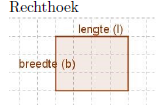
\includegraphics[width=5cm]{4_opp_inhoud_an_meetk/inputs/fig1.png}
%		\end{tabular}
		& $O=2(l+b)$ & $A=l.b$ \\
		\begin{tabular}{l}
		Vierkant \\
		\tikzsetfigurename{module4_1_vierkant}
		\begin{tikzpicture}
		\draw[draw=black,fill=yellow,fill opacity=0.2] (0,0) rectangle ++(2,2);
		\node[] at (1.25,2.5) { zijde $z$};
		\node[] at (-1,1.25) { zijde $z$};
		\end{tikzpicture} \end{tabular}
		& $O=4z$ & $A=z^2$ \\
		\begin{tabular}{l}
		Rechthoekige driehoek \\
		\tikzsetfigurename{module4_1_rechthoekigeDriehoek}
		\begin{tikzpicture}
		\node (r0) at ( 0.0,  0.0) {}; % root
		\node (s0) at ( 4.0,  0.0) {}; % extreme
		\node (s1) at ( 4.0,  3.0) {}; % extreme
		
		\draw[draw=black,fill=yellow!20] (r0.center)--(s0.center)--(s1.center) -- (r0.center);
%		draw (0,0) node[anchor=north]{$A$}
%		-- (5,0) node[anchor=north]{$C$}
%		-- (5,4) node[anchor=south]{$B$}
%		-- cycle;
		\node[] at (2,-0.5) {basis $b$};
		\node[] at (5,1.5) {hoogte $h$};
		\node[] at (0,1.5) {schuine zijde $s$};
		\end{tikzpicture} \end{tabular}
		& $O=b+h+s$ & $A=\frac{b.h}{2}$ \\
		\begin{tabular}{l}
		Niet-rechthoekige of willekeurige driehoek \\
		\tikzsetfigurename{module4_1_willekeurigeDriehoek}
		\begin{tikzpicture}
		\node (r0) at ( 0.0,  0.0) {}; % root
		\node (s0) at ( 4.0,  0.0) {}; % extreme
		\node (s1) at ( 1.0,  3.0) {}; % extreme
		
		\draw[draw=black,fill=yellow!20] (r0.center)--(s0.center)--(s1.center) -- (r0.center);
		\draw[dashed,draw=black] (s1.center)--(1,0);
		%		draw (0,0) node[anchor=north]{$A$}
		%		-- (5,0) node[anchor=north]{$C$}
		%		-- (5,4) node[anchor=south]{$B$}
		%		-- cycle;
		\node[] at (2,-0.5) {basis $b$};
		\node[] at (3,1.5) {$c$};
		\node[] at (0.2,1.5) {$a$};
		\node[anchor=south,right,xshift=-0.2cm] at (1,1.2) {hoogte $h$};
		\end{tikzpicture} \end{tabular}
		& $O=a+b+c$ & $A=\frac{b.h}{2}$ 
	\end{tabular}
\end{center}
\caption{Omtrek en oppervlakte van vlakke figuren (1).}
\label{tab:omtrek_opp1}
\end{sidewaystable}
\begin{table}
	\begin{center}
		\begin{tabular}{lll}
		Figuur & Omtrek & Oppervlakte \\
		\hline
		\begin{tabular}{l}
		Parallellogram \\
		\tikzsetfigurename{module4_1_parallellogram}
		\begin{tikzpicture}
		\node (r0) at ( 0.0,  0.0) {}; % root
		\node (s0) at ( 4.0,  0.0) {}; % extreme
		\node (s1) at ( 5.0,  3.0) {}; % extreme
		\node (s2) at ( 1.0,  3.0) {}; % extreme
		
		\draw[draw=black,fill=yellow!20] (r0.center)--(s0.center)--(s1.center) --(s2.center) -- (r0.center);
		\draw[dashed,draw=black] (s2.center)--(1,0);
		%		draw (0,0) node[anchor=north]{$A$}
		%		-- (5,0) node[anchor=north]{$C$}
		%		-- (5,4) node[anchor=south]{$B$}
		%		-- cycle;
		\node[] at (2,-0.5) {basis $b$};
		\node[] at (5,1.5) {$a$};
		\node[anchor=south,right] at (1,1.5) {hoogte $h$};
		\end{tikzpicture} \end{tabular}& $O=2(a+b)$ & $A=b.h$ \\
		\begin{tabular}{l}
		Trapezium \\
		\tikzsetfigurename{module4_1_trapezium}
		\begin{tikzpicture}
		\node (r0) at ( 0.0,  0.0) {}; % root
		\node (s0) at ( 4.0,  0.0) {}; % extreme
		\node (s1) at ( 3.0,  3.0) {}; % extreme
		\node (s2) at ( 1.0,  3.0) {}; % extreme
		
		\draw[draw=black,fill=yellow!20] (r0.center)--(s0.center)--(s1.center) --(s2.center) -- (r0.center);
		\draw[dashed,draw=black] (s2.center)--(1,0);
		%		draw (0,0) node[anchor=north]{$A$}
		%		-- (5,0) node[anchor=north]{$C$}
		%		-- (5,4) node[anchor=south]{$B$}
		%		-- cycle;
		\node[] at (2,-0.5) {$B$};
		\node[] at (2,3.5) {$b$};
		\node[] at (0,1.5) {$a$};
		\node[] at (4,1.5) {$c$};
		\node[anchor=south,right] at (1,1.5) {hoogte $h$};
		\end{tikzpicture} 		\end{tabular}
		& $O=a+b+c+B$ & \begin{tabular}{l}
			$A=\frac{b+B}{2}.h$ \\
			Als basis gebruiken we de gemiddelde breedte
		\end{tabular} \\
		\begin{tabular}{l}
		Schijf \\
		\tikzsetfigurename{module4_1_schijf}
		\begin{tikzpicture}
		\draw[draw=black, fill=yellow!20] (0,0) arc (0:360:1.5) ;
		\draw[] (-1.5,0) -- (-3,0) node[anchor=south,midway] {$r$};
		\end{tikzpicture}
		\end{tabular} & \begin{tabular}{l}
			$O=2\pi r$ \\
			Diameter $D=2.r$ \\
			$r$ is de straal
		\end{tabular} &
		\begin{tabular}{l}
			$A=\pi r^2$ \\
			$A=\frac{\pi D^2}{4}$
		\end{tabular} \\
		\begin{tabular}{l}
			Regelmatige $n$-hoek of veelhoek \\
			Bij zo'n veelhoek zijn alle zijden $z_n$ even lang \\
			en zijn alle hoeken even groot.\\
%			\begin{tikzpicture}[mystyle/.style={draw,shape=circle,fill=yellow!20}]
%			
%			\foreach \a in {5}{
%				\node [regular polygon, regular polygon sides=\a, minimum size=3cm, draw] at (\a*4,0) (A) {};
%%				\foreach \i in {1,...,\a}
%%				{%
%%					\node [label=90+72*(\i-1):\i, inner sep=1pt] at (A.corner \i) {};
%%				}
%			}
%%			\node[] at (0,0) {$z_n$};
%			
%%			\def\ngon{5}
%%			\node[regular polygon,regular polygon sides=\ngon,minimum size=3cm] (p) {};
%%			\foreach\x in {1,...,\ngon}{\node[mystyle] (p\x) at (p.corner \x){};}
%			
%			\end{tikzpicture}
			\tikzsetfigurename{module4_1_regelmatigeVeelhoek}
			\begin{tikzpicture}
			\polygon{5}{2}{1,2,3,4,5}{yellow!20};
			\node[anchor=south,below] (M) at (0,0) {$M$};
			\node[anchor=south,below] (A) at (0,2.2) {};
			\node[anchor=south,right] (R) at (0,1.1) {$R$};
			\node[anchor=south,below] (Z) at (0,-2) {$z_n$};
			\draw[dashed] (M) -- (A);
			\end{tikzpicture}
		\end{tabular} &
		\begin{tabular}{l}
			$O=n.z_n$ \\
			$O=n.2r.\sin(\frac{\pi}{n})$
		\end{tabular} & $A=n.r^2.\sin(\frac{\pi}{n}).\cos(\frac{\pi}{n})$
	\end{tabular}
\end{center}
\caption{Omtrek en oppervlakte van vlakke figuren (2).}
\label{tab:omtrek_opp2}
\end{table}
}

In de MOOC zie je een animatie die de formule voor de berekening van de oppervlakte van een trapezium verklaart.

\begin{minipage}{.25\linewidth}
	\raggedright
	
\includegraphics[width=4cm]{4_opp_inhoud_an_meetk/inputs/QR_Code_ANIMATIE_module4new}
\end{minipage}
\begin{minipage}{.7\linewidth}
	Scan de QR code om de animatie te bekijken.
\end{minipage}

\subsection{Ruimtefiguren}

\subsubsection{Prisma}
\begin{definitie}
	Een prisma is een ruimtefiguur waarvan twee zijvlakken evenwijdig zijn (bv. het grond- en bovenvlak) en de overige zijvlakken zijn evenwijdig met eenzelfde lijn die de evenwijdige vlakken snijdt.
\end{definitie} 
Een prisma wordt dus begrensd door twee evenwijdige en even grote veelhoeken (drie-, vier-, vijfhoeken,... ) die we het \emph{grondvlak en het bovenvlak} noemen. De \emph{opstaande zijvlakken} bestaan uit rechthoeken of parallellogrammen. De ribben die niet in het grond- of bovenvlak gelegen zijn hebben allen dezelfde lengte, we noemen ze de \emph{opstaande ribben}.

Naargelang het aantal opstaande zijvlakken spreken we van een driezijdig, vierzijdig, vijfzijdig,... prisma.

Een \emph{recht} prisma is een prisma, waarin de verbindende ribben en zijvlakken loodrecht op het grondvlak staan. Dit houdt in dat de verbindende zijvlakken rechthoeken zijn. Een scheef \emph{prisma} is een prisma, waarvan de verbindende ribben en zijvlakken niet loodrecht op het grondvlak staan. Dit houdt in dat de verbindende zijvlakken parallellogrammen zijn.

\gewonefiguur{width=.7\linewidth}{4_opp_inhoud_an_meetk/inputs/RuimteFigurenOppInhoud_prisma}

%\begin{figure}
%	\centering
%	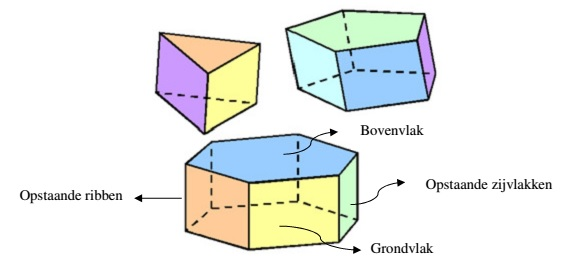
\includegraphics[width=0.7\linewidth]{4_opp_inhoud_an_meetk/inputs/RuimteFigurenOppInhoud_prisma}
%	\caption{Prisma.}
%	\label{fig:ruimtefigurenoppinhoudprisma}
%\end{figure}
		
\begin{ftonthoud}
		Oppervlakte van een prisma: $A=\text{opp}_{\text{grondvlak}}+\text{opp}_{\text{bovenvlak}}+\text{opp}_{\text{zijkanten}}$
		
		Volume van een prisma: $V=\text{opp}_{\text{grondvlak}}\cdot \text{hoogte}$
	
\end{ftonthoud}

We onderscheiden een drietal bijzondere prisma's.

\subsubsection{Kubus of hecta\"eder}
\begin{definitie}
	Elk zijvlak van de kubus vormt een vierkant.
\end{definitie}

Alle 8 ribben zijn dus even lang. Een kubus is een bijzonder recht prisma.

\gewonefiguur{width=.4\linewidth}{4_opp_inhoud_an_meetk/inputs/RuimteFigurenOppInhoud_kubus}

%\begin{figure}
%	\centering
%	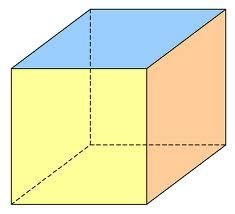
\includegraphics[width=0.7\linewidth]{4_opp_inhoud_an_meetk/inputs/RuimteFigurenOppInhoud_kubus}
%	\caption{Kubus}
%	\label{fig:ruimtefigurenoppinhoudkubus}
%\end{figure}

		
\begin{ftonthoud}
		Oppervlakte van een lubus: $A=6z^2$
		
		Volume van een kubus: $V=z^3$
\end{ftonthoud}
		

\subsubsection{Balk}
\begin{definitie}
	De 6 zijvlakken van de balk bestaan uit rechthoeken. 
\end{definitie}

Een balk is ook een bijzonder recht prisma.
Een balk is tevens een rechthoekig parallellepipedum.

\gewonefiguur{width=.7\linewidth}{4_opp_inhoud_an_meetk/inputs/RuimteFigurenOppInhoud_balk}

%\begin{figure}
%	\centering
%	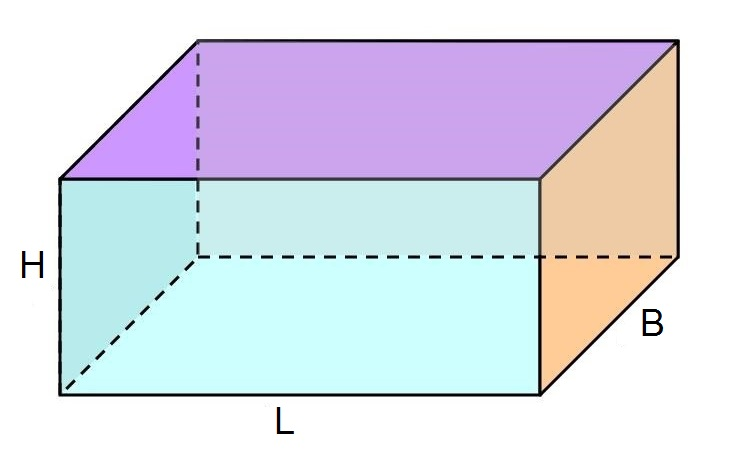
\includegraphics[width=0.7\linewidth]{4_opp_inhoud_an_meetk/inputs/RuimteFigurenOppInhoud_balk}
%	\caption{Balk.}
%	\label{fig:ruimtefigurenoppinhoudbalk}
%\end{figure}


\begin{ftonthoud}
			
		Oppervlakte van een prisma: $A=2(L\cdot B+B\cdot H+H\cdot L)$
		
		Volume van een prisma: $V=L\cdot B\cdot H$

\end{ftonthoud}

\subsubsection{Parallellepipedum}
\begin{definitie}
	Een parallellepipedum is een veelvlak waarvan alle 6 zijvlakken bestaan uit parallellogrammen die paarsgewijs gelijk en evenwijdig zijn. Dus ook het grond- en het bovenvlak zijn parallellogrammen. 

\end{definitie}
Een parallellepipedum is een bijzonder scheef prisma, terwijl de kubus en de balk speciale gevallen zijn van een parallellepipedum.

\gewonefiguur{width=.7\linewidth}{4_opp_inhoud_an_meetk/inputs/RuimteFigurenOppInhoud_parallellepipedum}

%\begin{figure}
%	\centering
%	\includegraphics[width=0.7\linewidth]{\gewonefiguur{width=.7\linewidth}{4_opp_inhoud_an_meetk/inputs/RuimteFigurenOppInhoud_balk}}
%	\caption{Parallellepipedum.}
%	\label{fig:ruimtefigurenoppinhoudparallellepipedum}
%\end{figure}


\begin{ftonthoud}
			
		Oppervlakte van een prisma: $A=\text{som van de oppervlakten}$
		
		Volume van een prisma: $V=\text{opp}_{\text{grondvlak}}\cdot \text{hoogte}$

\end{ftonthoud}		

\subsubsection{Piramide}
\begin{definitie}
	Een piramide is een ruimtefiguur waarvan het grondvlak een veelhoek (driehoek, vierhoek, vijfhoek, $\ldots$) is en waarvan de hoekpunten verbonden worden met een willekeurig punt in de ruimte. Dit punt noemen we de top van de piramide. De opstaande zijvlakken zijn allemaal driehoekig. 

\end{definitie}
Een rechte piramide heeft als grondvlak een regelmatige veelhoek en de top ligt boven het centrum van het grondvlak. Alle zijvlakken hebben dezelfde driehoekige vorm.

\gewonefiguur{width=.7\linewidth}{4_opp_inhoud_an_meetk/inputs/piramide}
%
%\begin{figure}
%	\centering
%	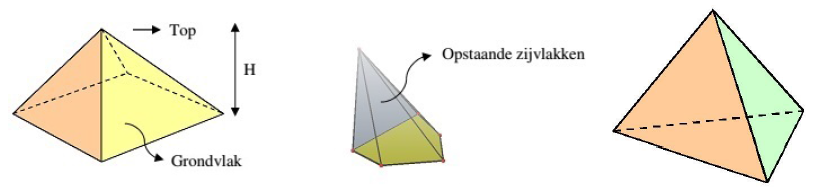
\includegraphics[width=0.7\linewidth]{4_opp_inhoud_an_meetk/inputs/piramide}
%	\caption{Piramide.}
%	\label{fig:piramide}
%\end{figure}



\begin{ftonthoud}
	Oppervlakte: $A=$ som van alle oppervlakten
\\
Volume: $V=\frac{1}{3}\text{opp}_{\text{grondvlak}}\cdot \text{hoogte}$
\end{ftonthoud}

\begin{definitie}
	Een \emph{tetra\"eder of viervlak} is een ruimtefiguur bestaande uit vier driehoekige vlakken. Het is dus een piramide met een driehoekig grondvlak.

Een \emph{regelmatig viervlak} bestaat uit vier gelijkbenige driehoeken.

\end{definitie}

\subsection{Omwentelingslichamen}

Deze lichamen hebben ten minste \'e\'en grensvlak dat niet vlak is. We noemen dit vlak een gebogen vlak of zijdelingsoppervlak of manteloppervlak. Omwentelingslichamen ontstaan door het wentelen van een vlak rond een rechte. Deze rechte noemen we dan de omwentelingsas.

\subsubsection{Cilinder}
\begin{definitie}
	Een cilinder is een lichaam dat ontstaat wanneer we een rechthoek met afmetingen  $R$ en $H$ om n van zijn zijden laten wentelen.
\end{definitie}
 Beschouw de omwentelingscilinder, met $R$ als de straal van het grond- en bovenvlak en $H$ als de hoogte.

Het grond- en bovenvlak zijn twee evenwijdige schijven met de zelfde straal $R$. De afstand tussen (de middelpunten van) het grond- en bovenvlak noemen we de hoogte $H$. Bij een \emph{rechte cilinder} staat de omwentelingsas loodrecht op het grondvlak, zo niet dan spreken we van een \emph{scheve cilinder}.

De totale oppervlakte van de cilinder is gelijk aan de som van de oppervlakten van het grond- en het bovenvlak (= oppervlakte schijf is $\pi R^2$) en de zijdelingse oppervlakte (= een rechthoek met oppervlakte $2\pi R\cdot H$). De inhoud van de cilinder is het product van oppervlakte grondvlak met de hoogte.

\gewonefiguur{width=.7\linewidth}{4_opp_inhoud_an_meetk/inputs/RuimteFigurenOppInhoud_parallellepipedum}

%\begin{figure}[h]
%	\centering
%	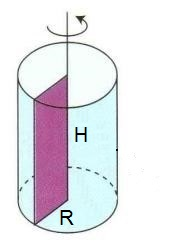
\includegraphics[width=0.3\linewidth]{4_opp_inhoud_an_meetk/inputs/RuimteFigurenOppInhoud_cilinder1}
%	\caption{Cilinder}
%	\label{fig:ruimtefigurenoppinhoudcilinder1}
%\end{figure}

\begin{ftonthoud}
	
		Oppervlakte: $A=2\pi R^2 + 2\pi RH$
		\\
		Volume: $V=\pi R^2 H$
\end{ftonthoud}

\subsubsection{Kegel}
\begin{definitie}
	Een kegel is het lichaam dat ontstaat als we een rechthoekige driehoek laten wentelen om \'e\'en van zijn rechthoekszijden. Het grondvlak van de kegel is een schijf met straal $R$. De afstand van de top tot het middelpunt van het grondvlak noemen we de hoogte $H$ van de kegel. Het apothema $a$ van de kegel is de lengte van het lijnstuk $[AB]$, we spreken ook wel van de schuine hoogte.
\end{definitie}
De lengte van het apothema kan gemakkelijk berekend worden a.d.h.v. de stelling van Pythagoras: $a=R+H$.

De totale oppervlakte van de kegel is gelijk aan de som van de oppervlakte van het grondvlak (= oppervlakte schijf is $\pi R^2$) en de zijdelingse oppervlakte ($\pi R a$). De inhoud van de kegel is het product van oppervlakte grondvlak met de hoogte en de constante.

\gewonefiguur{width=.7\linewidth}{4_opp_inhoud_an_meetk/inputs/RuimteFigurenOppInhoud_kegel1}

%\begin{figure}[h]
%	\centering
%	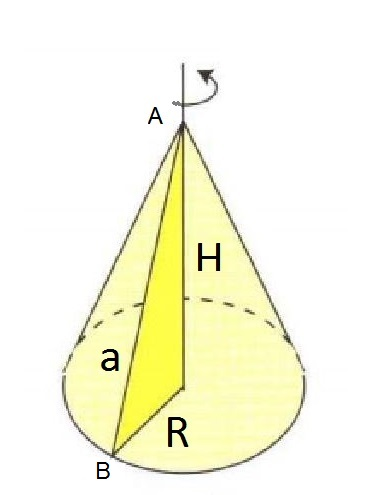
\includegraphics[width=0.3\linewidth]{4_opp_inhoud_an_meetk/inputs/RuimteFigurenOppInhoud_kegel1}
%	\caption{Kegel}
%	\label{fig:ruimtefigurenoppinhoudkegel1}
%\end{figure}


		
\begin{ftonthoud}
			Oppervlakte: $A=\pi R^2 + \pi R a$ 
		\\
		Volume: $V=\frac{1}{3}\pi R^2 H$
\end{ftonthoud}

\subsubsection{Bol}
\begin{definitie}
	Een bol is het lichaam dat ontstaat als we een schijf laten wentelen om de middellijn.
\end{definitie} Een bol heeft maar \'e\'en zijvlak, we spreken van het boloppervlak. 
Alle punten van het boloppervlak liggen op dezelfde afstand van het middelpunt. Deze afstand noemen we de straal $R$.

\gewonefiguur{width=.3\linewidth}{4_opp_inhoud_an_meetk/inputs/RuimteFigurenOppInhoud_bol1}

%\begin{figure}[h]
%	\centering
%	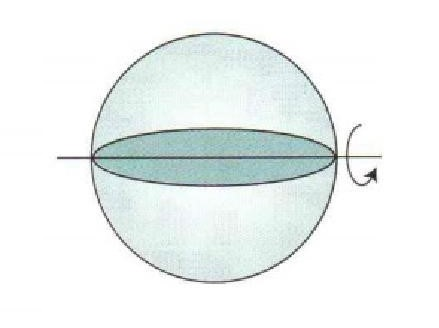
\includegraphics[width=0.3\linewidth]{4_opp_inhoud_an_meetk/inputs/RuimteFigurenOppInhoud_bol1}
%	\caption{Bol}
%	\label{fig:ruimtefigurenoppinhoudbol1}
%\end{figure}


		
\begin{ftonthoud}
			Oppervlakte: $A=4\pi R^2$
		\\
		Volume: $V=\frac{4}{3}\pi R^3$
\end{ftonthoud}


\subsection{Test oppervlakte en inhoudsberekeningen}
TODO